\documentclass{beamer}

\usepackage[utf8]{inputenc}
\usepackage[T1]{fontenc} % Allows bold italic text in title

\usepackage{array}

%\usetheme{Berlin}
%\usecolortheme{spruce}

\usetheme[progressbar=frametitle]{metropolis}
%\setbeamertemplate{frame numbering}[fraction]
\setbeamertemplate{frame numbering}[none]
\useoutertheme{metropolis}
\useinnertheme{metropolis}
\usefonttheme{metropolis}
\usecolortheme{spruce}
\setbeamercolor{background canvas}{bg=white}

%\setbeamertemplate{section in toc}[ball unnumbered]
%\setbeamertemplate{subsection in toc}[ball unnumbered]
\setbeamertemplate{section in toc}[sections numbered]
\setbeamertemplate{subsection in toc}[subsections numbered]

\title{Al Loro: \\Lector de \textit{feeds RSS} para asistente de voz}
\author[Alejandro Gómez Noé]{\emph{Autor:} Alejandro Gómez Noé\\[0.3em]\emph{Tutor:} Vicente Pelechano Ferragud}
\institute{ETSINF - Universidad Politécnica de Valencia}
\date{Curso 2020-2021}

\begin{document}
  
  \begin{frame}[noframenumbering,plain]
    \titlepage
  \end{frame}
  
  \begin{frame}[noframenumbering,plain]{Índice general}
    \tableofcontents
  \end{frame}

  \section{Introducción}
 
  \begin{frame}{¿Qué es Alexa?}
    \begin{columns}[c]
      \begin{column}{.51\textwidth}
        \begin{itemize}
          \setlength\itemsep{1.5em}
          \only<1>
          {
          \item Alexa es un \textbf{asistente de voz}
          \item Es un servicio de \textbf{Amazon}
          \item Puede obtener información como el \textbf{tiempo}, el \textbf{tráfico}, o las \textbf{noticias}
          }
          \only<2>
          {
          \item Disponible en \textbf{dispositivos Echo} y \textbf{móviles}
          \item Integración con \textbf{domótica}
          \item Permite a los desarrolladores crear \textbf{aplicaciones} (\textbf{\emph{skills}})
          }
        \end{itemize}
      \end{column}
      \begin{column}{.49\textwidth}
        \only<1>
        {
          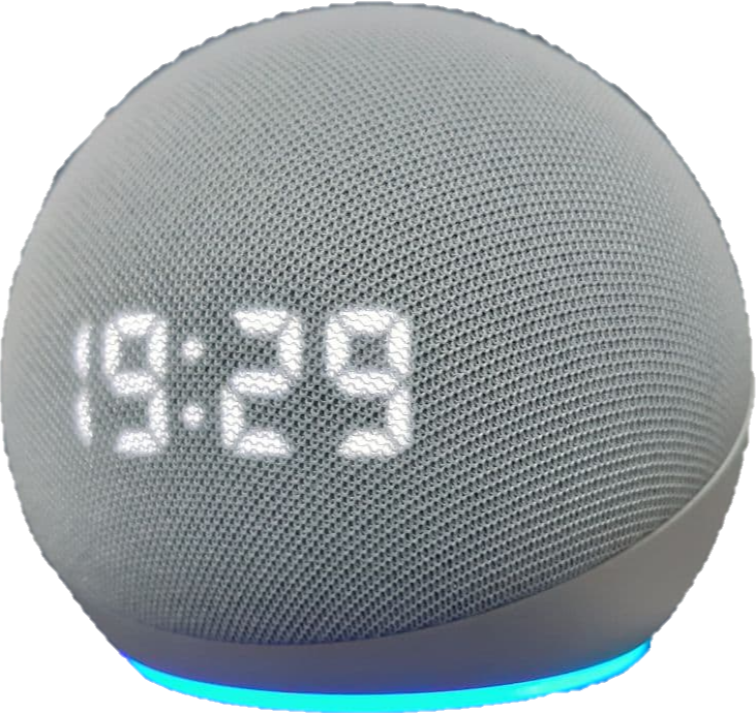
\includegraphics[width=.46\textwidth]{echo-dot.png}
          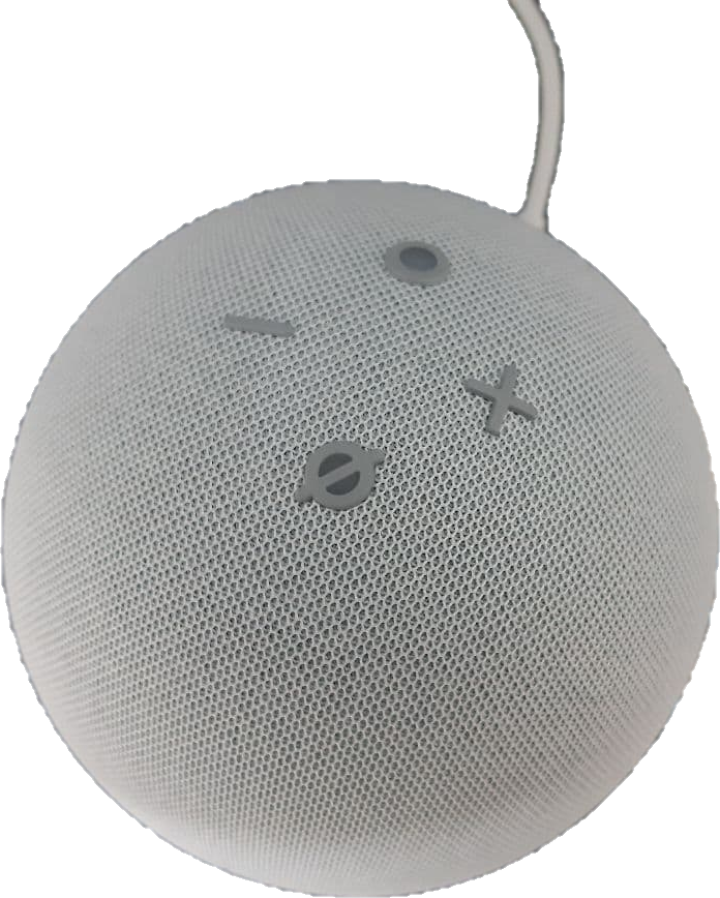
\includegraphics[width=.46\textwidth]{echo-dot-2.png}
          \centering
          {
          \footnotesize
          Dispositivo Amazon Echo Dot\\
          (4ª Generación, con reloj)
          }
        }
        \only<2>
        {
          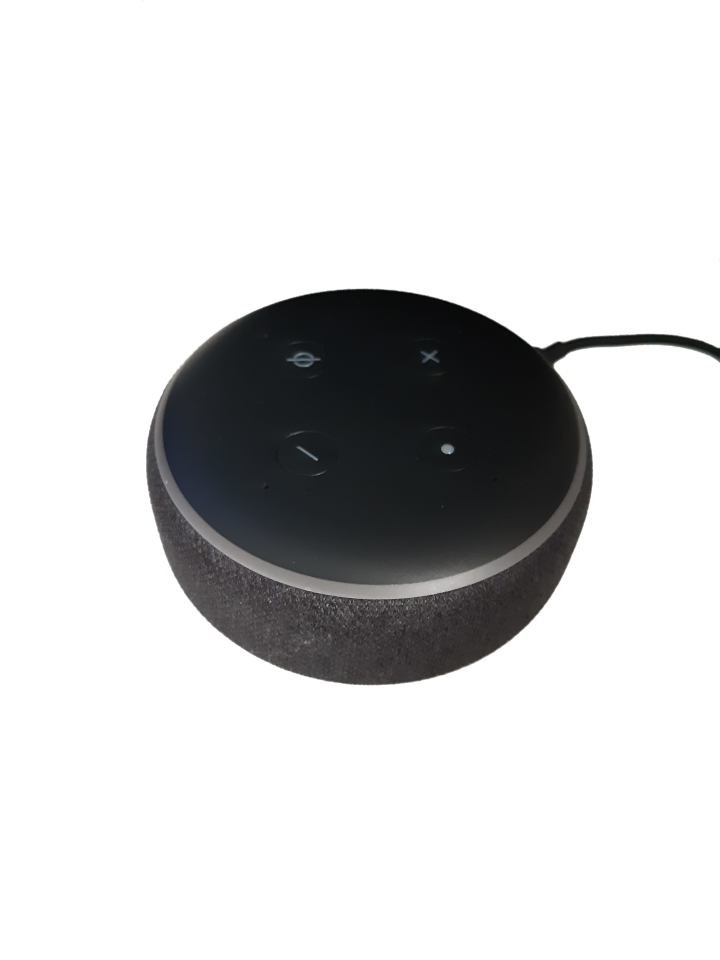
\includegraphics[width=\textwidth,trim={0 45cm 0 40cm},clip]
          {echo-dot-3-gen.png}
          \centering
          {
          \footnotesize
          Dispositivo Amazon Echo Dot\\
          (3ª Generación)
          }
        }
        
      \end{column}
    \end{columns}
  \end{frame}

  \begin{frame}{¿Qué es una feed?}
    \only<1>
    {
      \begin{itemize}
        \setlength\itemsep{1.5em}
        \item Las \textbf{feeds} son \textbf{listados} que se \textbf{actualizan periódicamente}
        \item Suelen estar alojadas en una \textbf{página web}
        \item Habitual en sitios de \textbf{noticias}, \textbf{blogs}, \textbf{podcasts}\dots
      \end{itemize}
    }
    \only<2>
    {
      Alexa tiene un \textbf{sistema de noticias} que soporta los siguientes formatos:

      \vspace{2em}

      \begin{columns}[t]
        \begin{column}{.49\textwidth}
          \centering
          \hyperlink{rss}{
\includegraphics{rss-logo.png}}\\[.5em]
          \textbf{RSS}\\{\footnotesize(\textit{Really Simple Syndication})}
        \end{column}
        \begin{column}{.49\textwidth}
          \centering
          
\includegraphics[scale=.8]{json-logo.png}\\[.5em]
          JSON
        \end{column}
      \end{columns}
    }
  \end{frame}

  \begin{frame}[label=rss]{RSS}
    \only<1>
    {
      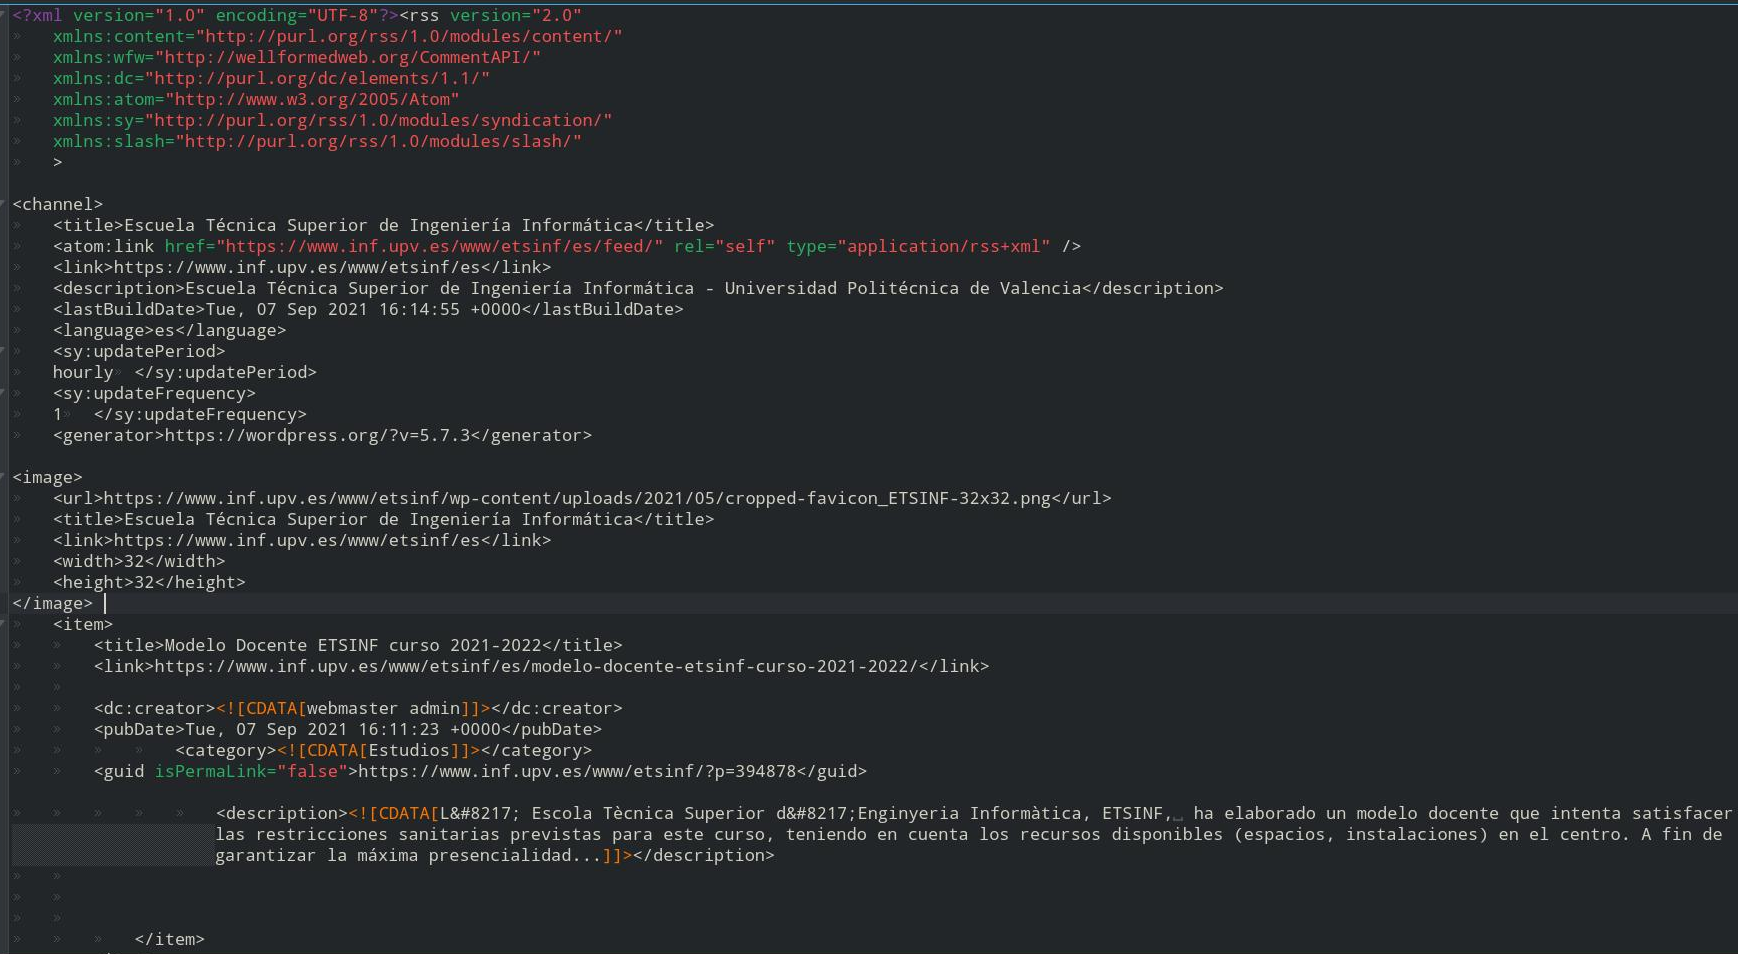
\includegraphics[width=\textwidth,trim={0 0 13.5cm 0},clip]{rss-feed-example.png} 
    }
    \only<2>
    {
      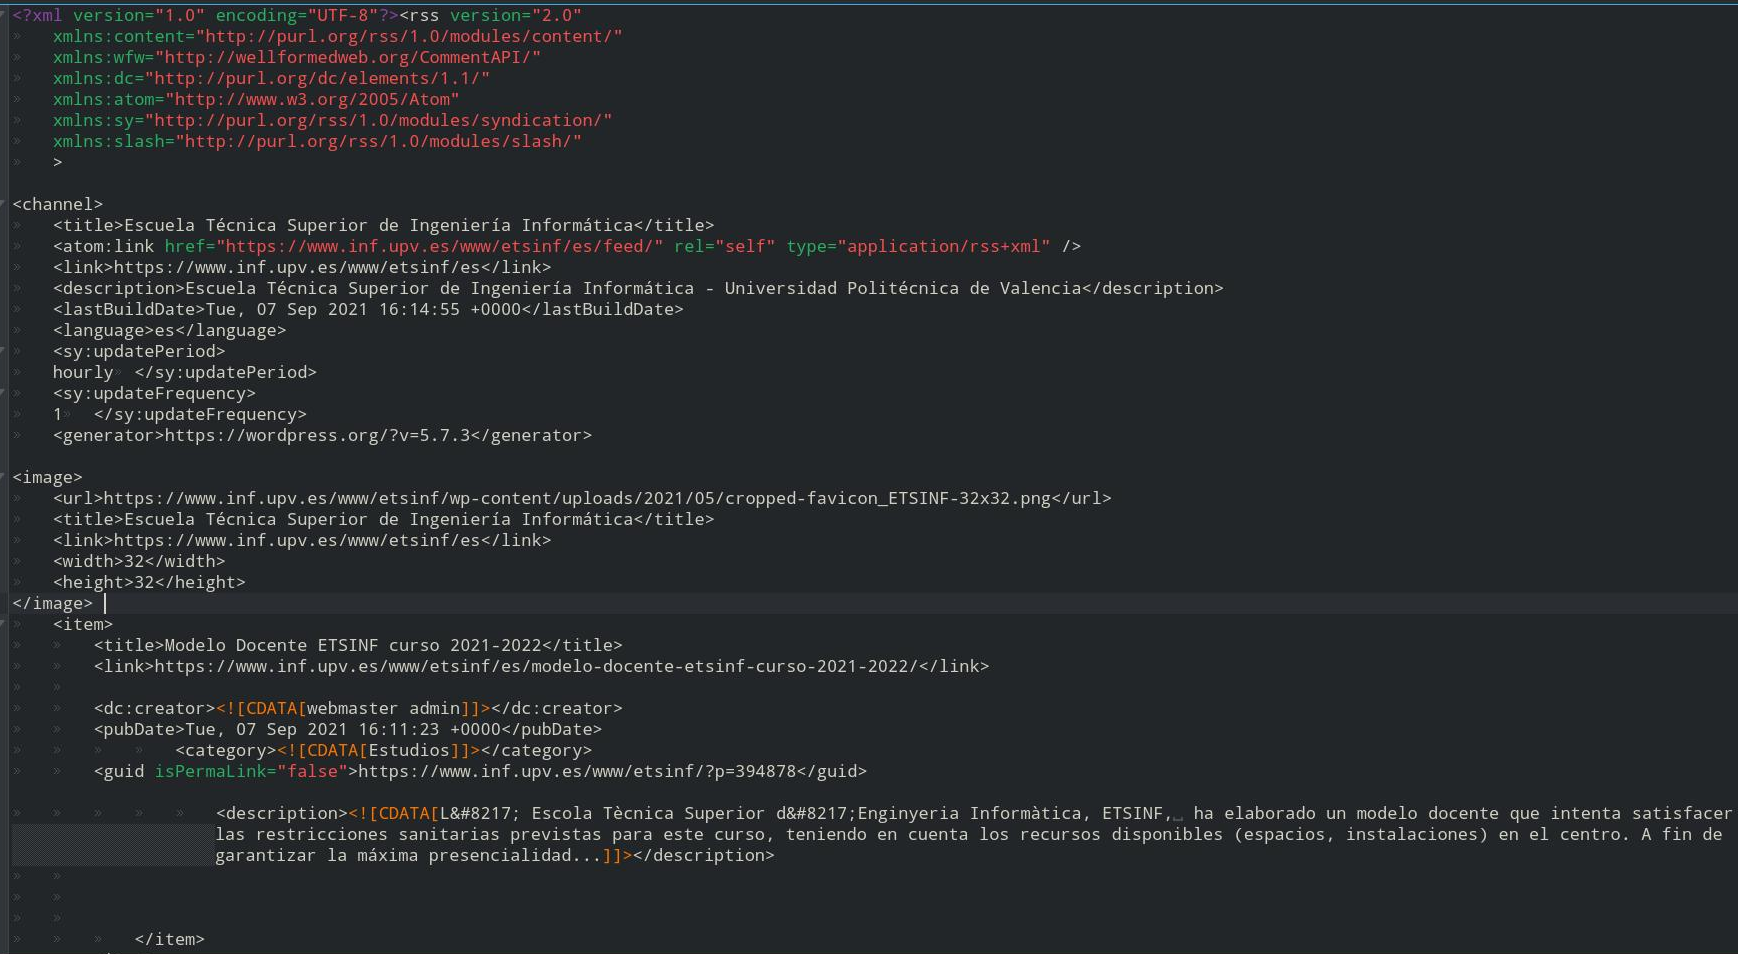
\includegraphics[width=\textwidth,trim={0 9cm 13.5cm 5cm},clip]{rss-feed-example.png} 
      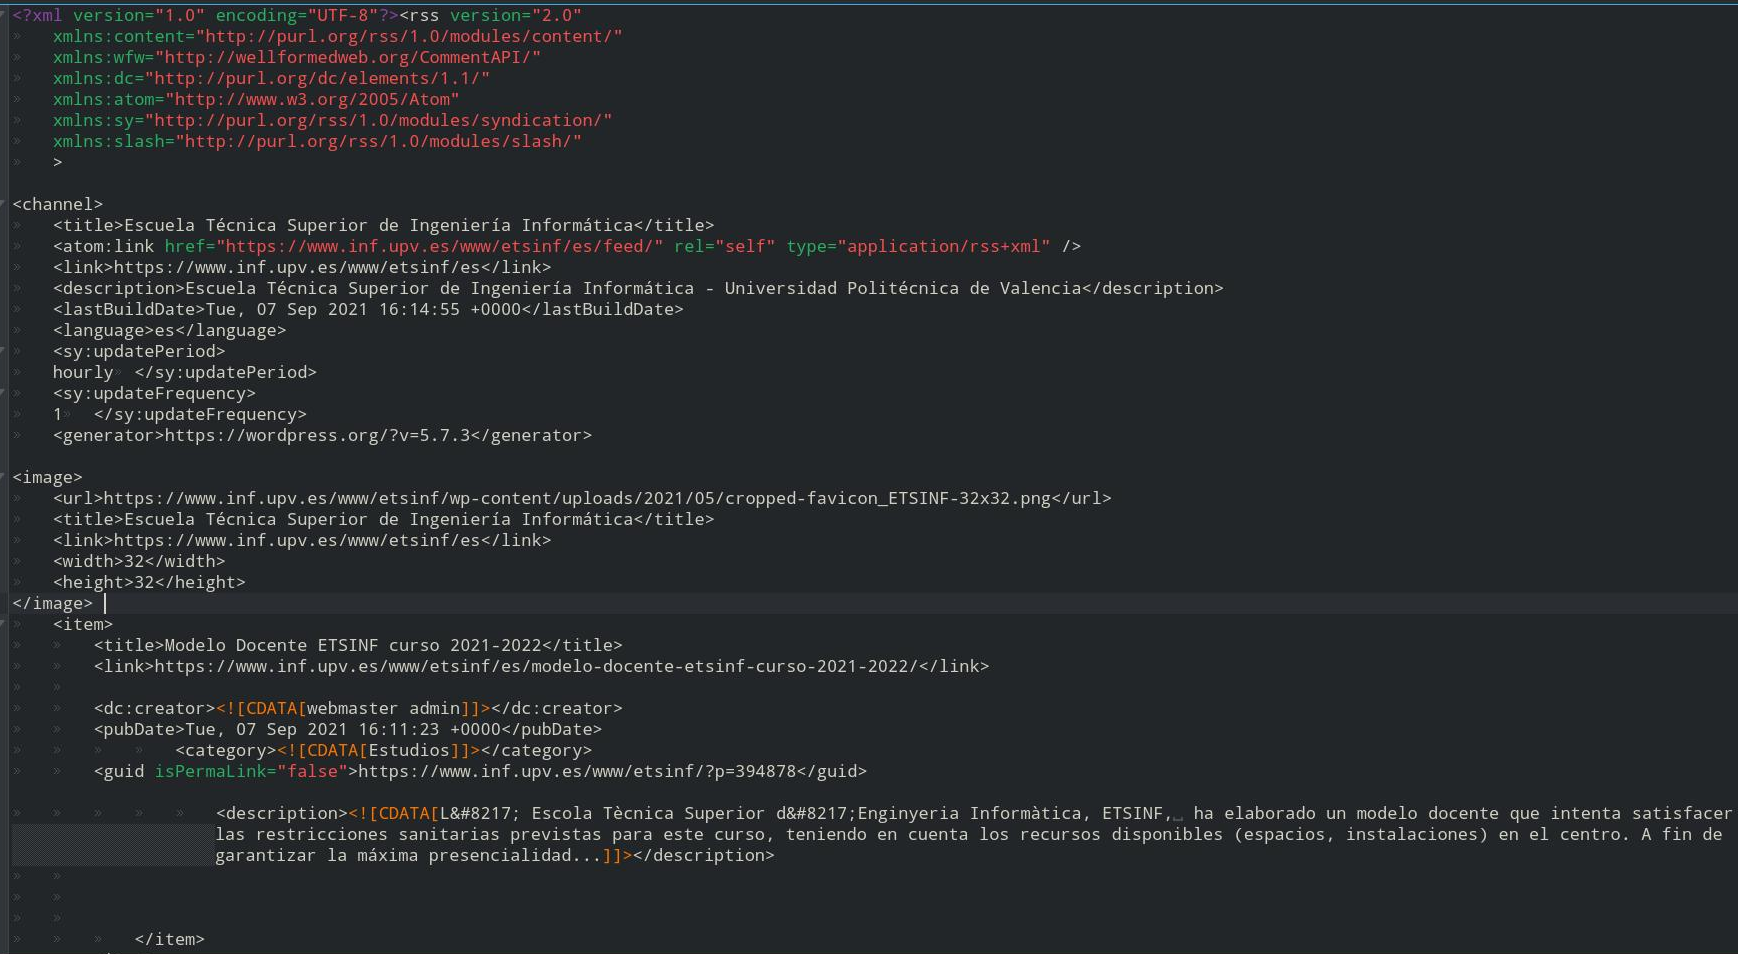
\includegraphics[width=\textwidth,trim={0 0 19.75cm 16.3cm},clip]{rss-feed-example.png} 
    }
  \end{frame}

  \section{Motivación}
  
  \newcommand{\includecenteredgraphicsb}[3][.35]{\raisebox{-#1\height}{\includegraphics[scale=#2]{#3}}}
  \newcommand{\includecenteredgraphicsl}[3][.35]{\includecenteredgraphicsb[#1]{#2}{#3}\hspace{.1em}}
  \newcommand{\includecenteredgraphicsr}[3][.35]{\hspace{.1em}\includecenteredgraphicsb[#1]{#2}{#3}}
 
  \begin{frame}{Motivación}
    \begin{itemize}
      \setlength\itemsep{1.5em}
      \item Entender más sobre los \textbf{servicios en la nube}
      \includecenteredgraphicsr{.35}{aws-lambda-logo.png}
      \item Aprender un lenguaje de programación (\textbf{TypeScript})
      \includecenteredgraphicsr{.02}{typescript-logo.png}
      \item Introducirme en un campo nuevo (\textbf{asistentes de voz})
      \includecenteredgraphicsr{1}{amazon-alexa.png}
    \end{itemize}
  \end{frame}

  \section{Estado del arte}

  \begin{frame}[c]{Asistentes de voz más populares}
    \vspace{1em}
    \begin{columns}[c]
      \begin{column}{.5\textwidth}
        \centering
        \hyperlink{asistente-google}{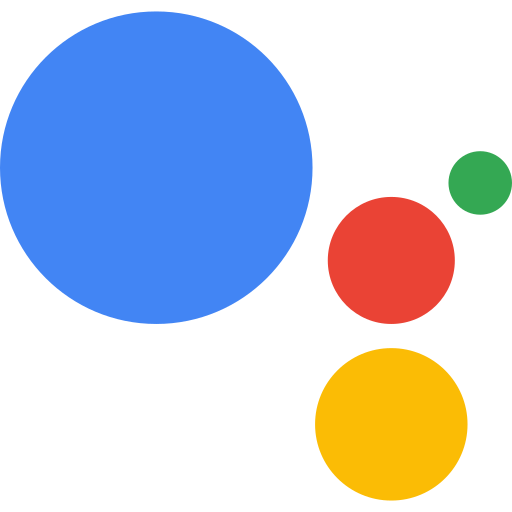
\includegraphics[scale=.207]{asistente-google-logo.png}}\\
        Asistente de Google
      \end{column}
      \begin{column}{.5\textwidth}
        \centering
        \hyperlink{amazon-alexa}{
\includegraphics[scale=4.3]{amazon-alexa.png}}\\
        Amazon Alexa
      \end{column}
    \end{columns}

    \vspace{2em}

    \begin{columns}
      \begin{column}{\textwidth}
        \centering
        \hyperlink{apple-siri}{
\includegraphics[scale=.4]{apple-siri-logo.png}}\\
        (Apple) Siri
      \end{column}
    \end{columns}
  \end{frame}

  \begin{frame}[label=asistente-google]{\includecenteredgraphicsl{.05}{asistente-google-logo.png} Asistente de Google}
    \only<1>
    {
      \textbf{Ventajas:}
      \vspace{1.5em}
      \begin{itemize}
        \setlength\itemsep{1.5em}
        \item Uno de los \textbf{más populares en el mercado}
        \item Instalado por defecto en \textbf{Android}
        \item Sistema de \textbf{búsqueda por internet}
      \end{itemize}
    }
    \only<2>
    {
      Kit de desarrollo: \textbf{\emph{Google Actions}}
      \begin{itemize}
        \item Enfocado a desarrolladores \textbf{principiantes}
        \item \textbf{Herramienta} de modelado basada en \textbf{diagramas}
        \item Para desarrolladores avanzados: \textbf{\textit{webhooks}}
      \end{itemize}
      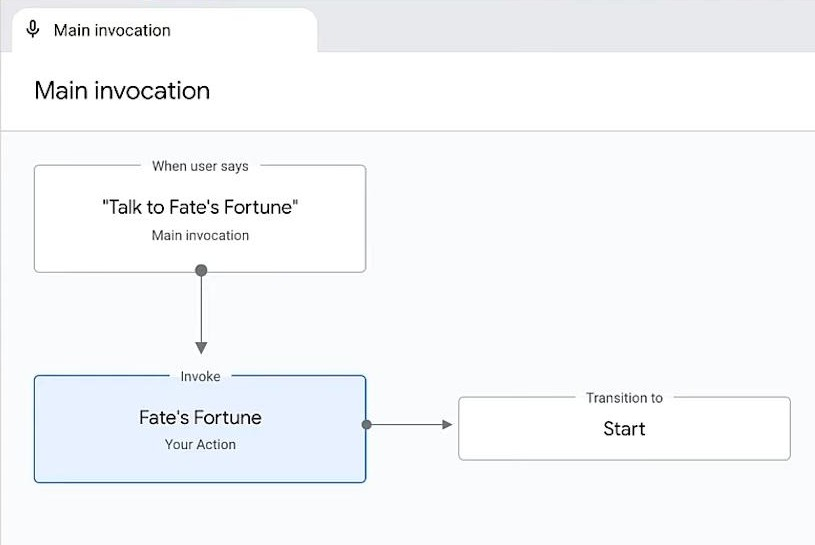
\includegraphics[scale=.4]{google-actions-console.jpg}
    }
  \end{frame}

  \begin{frame}[label=amazon-alexa]{\includecenteredgraphicsl[.22]{.8}{amazon-alexa.png} Amazon Alexa}
    \only<1>
    {
      \textbf{Ventajas:}
      \vspace{1.5em}
      \begin{itemize}
        \setlength\itemsep{1.5em}
        \item Muy \textbf{popular} entre los dispositivos \textbf{\textit{Smart Home}}
        \item \textbf{Integración} con otras \textbf{plataformas}
        \item Alto nivel de \textbf{inversión} en las \textbf{\emph{skills}}
      \end{itemize}
    }
    \only<2>
    {
      \textbf{Inconvenientes:}
      \vspace{1.5em}
      \begin{itemize}
        \item Sistema de \textbf{búsqueda por internet}\\
        \vspace{.5em}
        {\small Su porcentaje de respuestas sin responder es de un 23\%, mientras que la de los demás asistentes no llega al 10\%}\\
        \vspace{.3em}
        {\footnotesize(Estudio: \textit{SEMrush}, 2020)}
      \end{itemize}
    }
    \only<3>
    {
      \textbf{Categorías} de \textbf{skills} más destacadas:
      \vspace{1.5em}
      \begin{itemize}
        \setlength\itemsep{1.5em}
        \item \textbf{Entretenimiento}: Juegos y curiosidades, cuentos para niños, meditación, recetas de cocina\dots
        \item \textbf{Hogar digital} (\textit{Smart Home}): Bombillas inteligentes, cámaras de vigilancia, o termostatos.
        \item \textbf{Multimedia}: Cadenas de radio o \textit{podcasts}.
        \item \textbf{Noticias}: Televisión, radio, YouTube\dots
     \end{itemize}
    }
    \only<4>
    {
      Kit de desarrollo: \textbf{\emph{Alexa Skills}}
      \vspace{.7em}
      \begin{itemize}
        \setlength\itemsep{1.5em}
        \item Curva de aprendizaje intermedia
        \item Enfocado a \textbf{desarrolladores web}
        \item \textbf{Soporte} para \textbf{lenguajes muy utilizados} (\emph{JavaScript, Python})
      \end{itemize}
    }
  \end{frame}

  \begin{frame}[label=apple-siri]{\includecenteredgraphicsl{.1}{apple-siri-logo.png} (Apple) Siri}
    \only<1>
    {
      \textbf{Ventajas:}
      \vspace{1.5em}
      \begin{itemize}
        \setlength\itemsep{1.5em}
        \item \textbf{Muy popular} entre \textbf{usuarios} de productos \textbf{\emph{Apple}}
        \item Mayor \textbf{integración} con \textbf{apps} de \textbf{\emph{iOS}}
        \item Enfoque en la \textbf{productividad}
      \end{itemize}
    }
    \only<2>
    {
      \textbf{Inconvenientes:}
      \vspace{1.5em}
      \begin{itemize}
        \setlength\itemsep{1.5em}
        \item \textbf{Exclusivo} de productos \textbf{\emph{Apple}} {\small(menor cuota de mercado)}
        \item \textbf{Aplicaciones} personalizadas \textbf{requieren} una \textbf{app} para \textbf{\emph{iOS}}
        \item \textbf{Alta complejidad} para \textbf{desarrollar aplicaciones}
      \end{itemize}
    }
    \only<3>
    {
      Kit de desarrollo: \textbf{\emph{SiriKit}}
      \vspace{.7em}
      \begin{itemize}
        \setlength\itemsep{1.5em}
        \item Fuertemente acoplado al sistema de \textbf{\textit{iOS}}
        \item \textbf{Menos abierto} a nuevos desarrolladores
        \item \textbf{Requisitos muy específicos}:
        \vspace{.5em}
          \begin{itemize}
            \setlength\itemsep{.7em}
            \item Conocimientos en el lenguaje \textbf{\emph{Swift}} (propio de \emph{Apple})
            \item Un \textbf{ordenador} de la familia \textbf{\emph{Mac}}
            (acceso al editor \emph{XCode})
          \end{itemize}
      \end{itemize}
    }
  \end{frame}

  \begin{frame}[c]{Tabla comparativa}
    \begin{tabular}{@{}|>{\raggedright\small}p{0.22\linewidth}|>{\raggedright\small}p{0.22\linewidth}|>{\raggedright\small}p{0.22\linewidth}|>{\raggedright\arraybackslash\small}p{0.22\linewidth}| @{}}
      \hline
      & \normalsize Google \includecenteredgraphicsr[.25]{.03}{asistente-google-logo.png} & \normalsize \textbf{Alexa} \includecenteredgraphicsr[.25]{.65}{amazon-alexa.png} & \normalsize Siri \includecenteredgraphicsr[.25]{.06}{apple-siri-logo.png} \\
      \hline
      Kits de desarrollo & \emph{Actions} & \emph{Skills} & \emph{SiriKit} \\
      \hline
      Lenguajes soportados & JavaScript (Node.js) & JavaScript (Node.js), Python & Swift, Objective-C \\
      \hline
      Plataformas & Android, Google Home & Amazon Echo, Fire TV, Android e iOS & iOS, HomePod \\
      \hline
      Mayor enfoque & Búsqueda por Internet & \emph{Skills}, domótica, entretenimiento & Productividad \\
      \hline 
    \end{tabular}
   %\caption{Comparativa de los asistentes de voz más populares}
  \end{frame}

  \section{Propuesta de solución}
 
  \begin{frame}{Propuesta de solución}
    Profundizar en aspectos de la creación de skills en Alexa:
    \vspace{1.5em}
    \begin{itemize}
      \setlength\itemsep{1.5em}
      \item Similitudes con el desarrollo \textbf{\emph{backend}}
      \item \textbf{Integrar} skill con otros \textbf{servicios} (\textbf{apps}, \textbf{bases de datos}, etc.)
      \item Funcionamiento de una \textbf{interfaz guiada por voz}
    \end{itemize}
  \end{frame}

  \begin{frame}{Creación de una skill}
    Crear una skill de ejemplo:
    \vspace{1.5em}
    \begin{itemize}
      \setlength\itemsep{1.5em}
      \item Nombre: \textbf{Al Loro}
      \item Tipo de skill: \textbf{Noticias}
      \item Objetivo: \textbf{Mejorar} la \textbf{integración} del sistema de \textbf{noticias} de \textbf{Alexa} con los \textbf{servicios actuales}
    \end{itemize}
  \end{frame}

  \section{Diseño, arquitectura, esquema de la solución realizada}

  \begin{frame}{Arquitectura del sistema}
    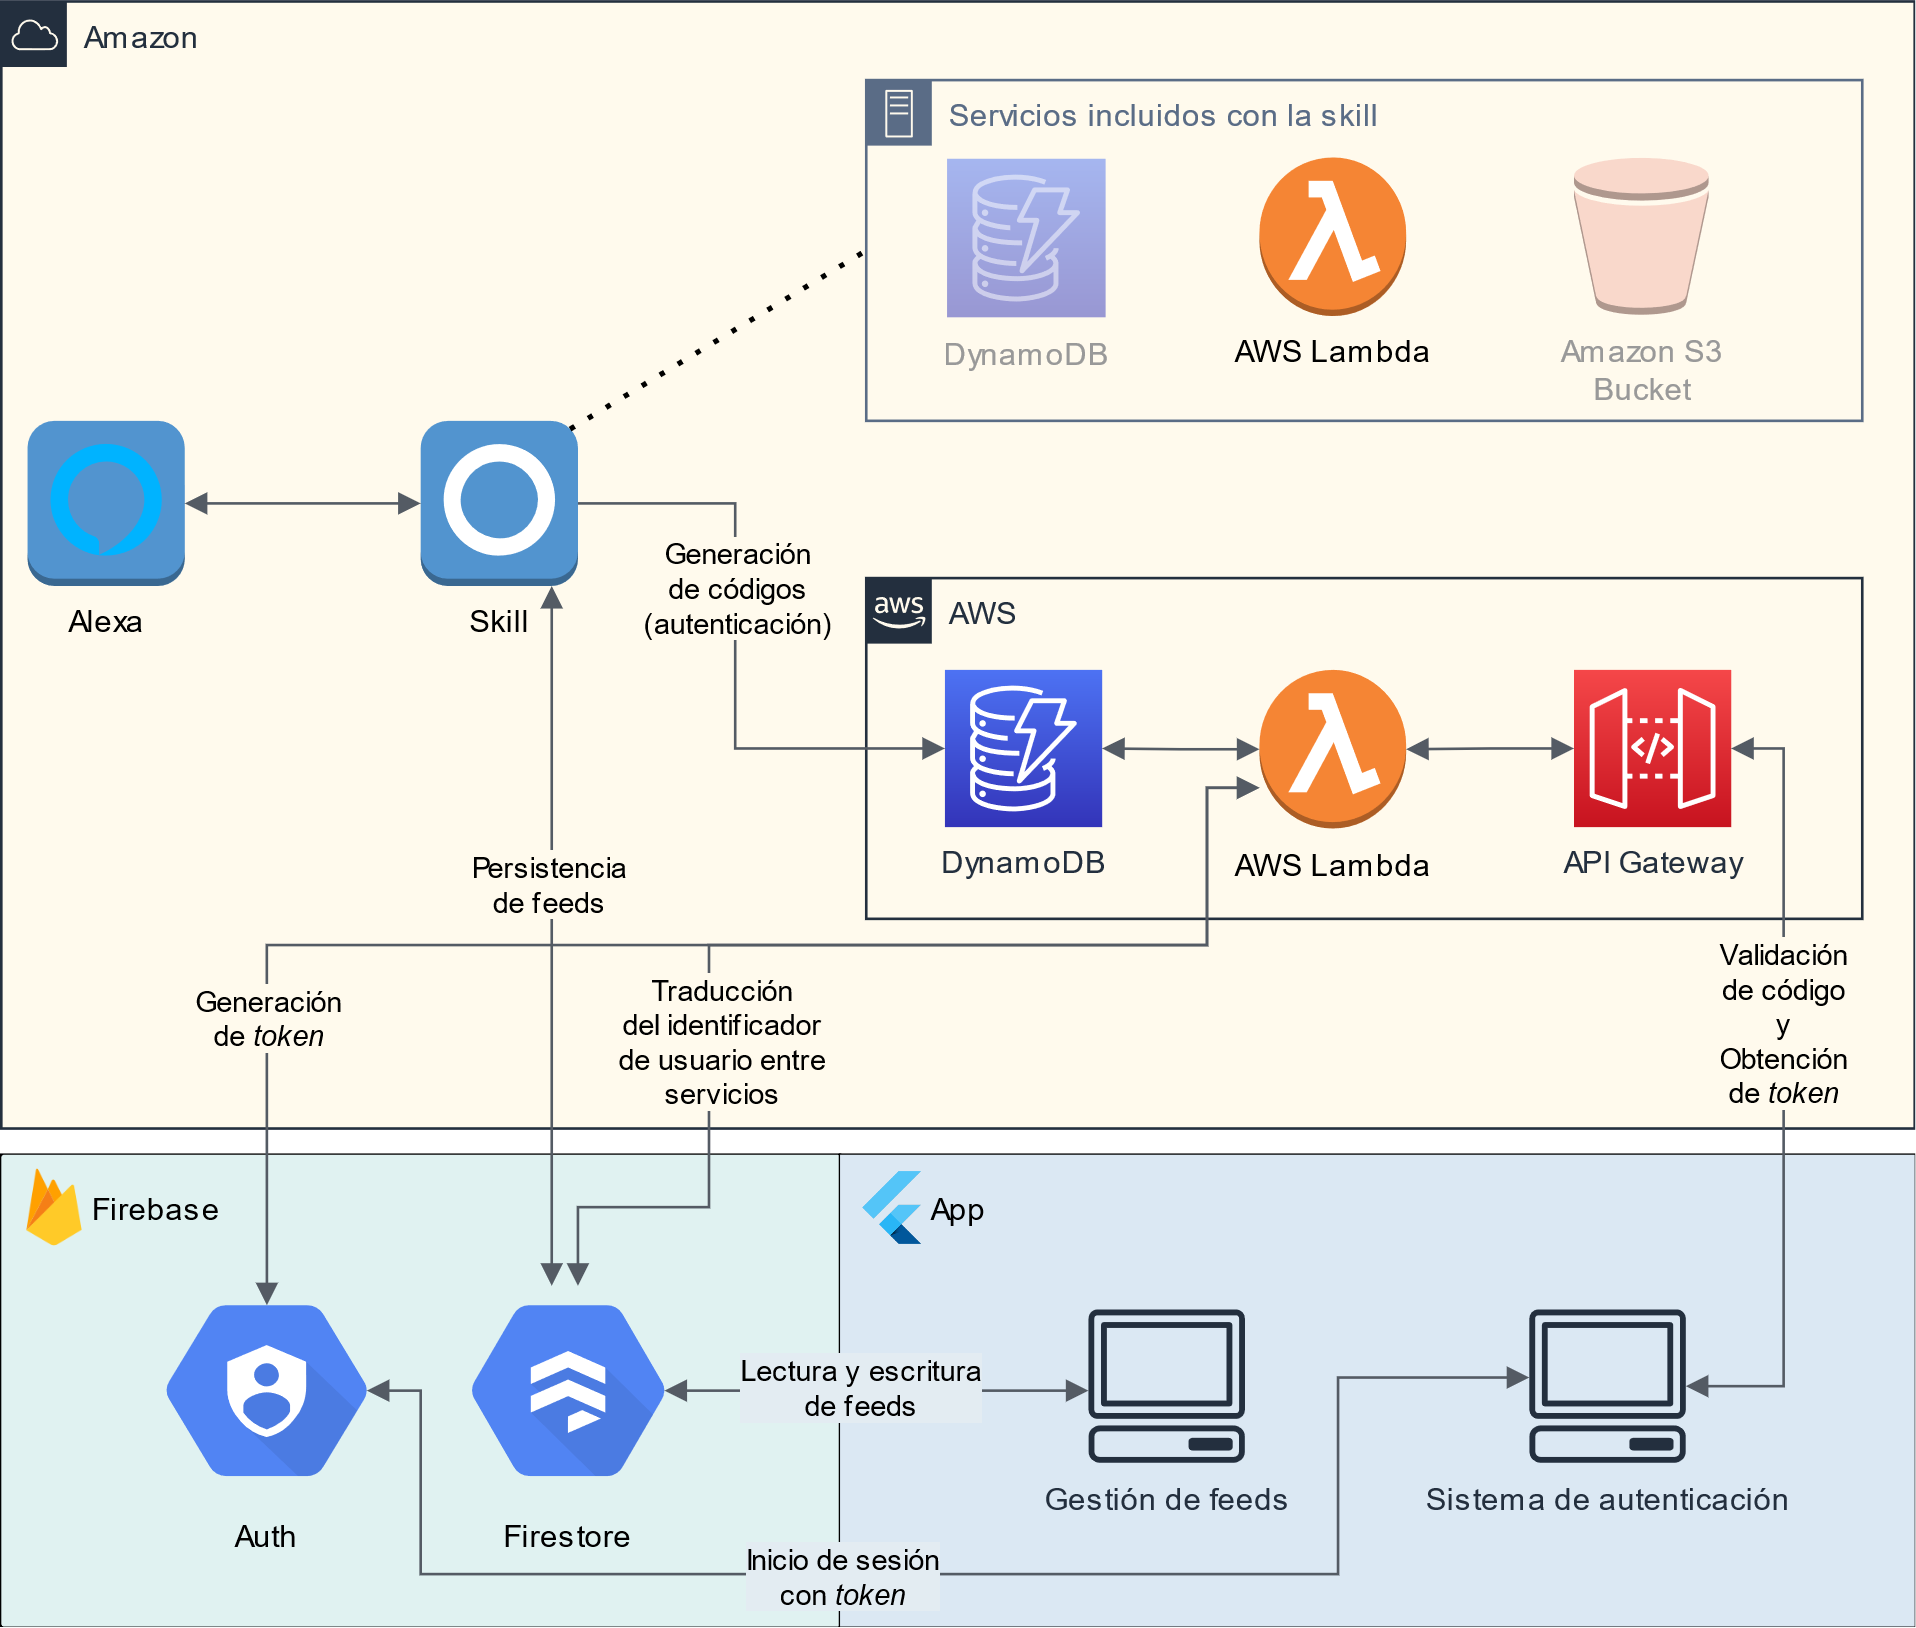
\includegraphics[width=.9\textwidth]{diagrama-bloques.png}  
  \end{frame}

  \begin{frame}{Skill}
    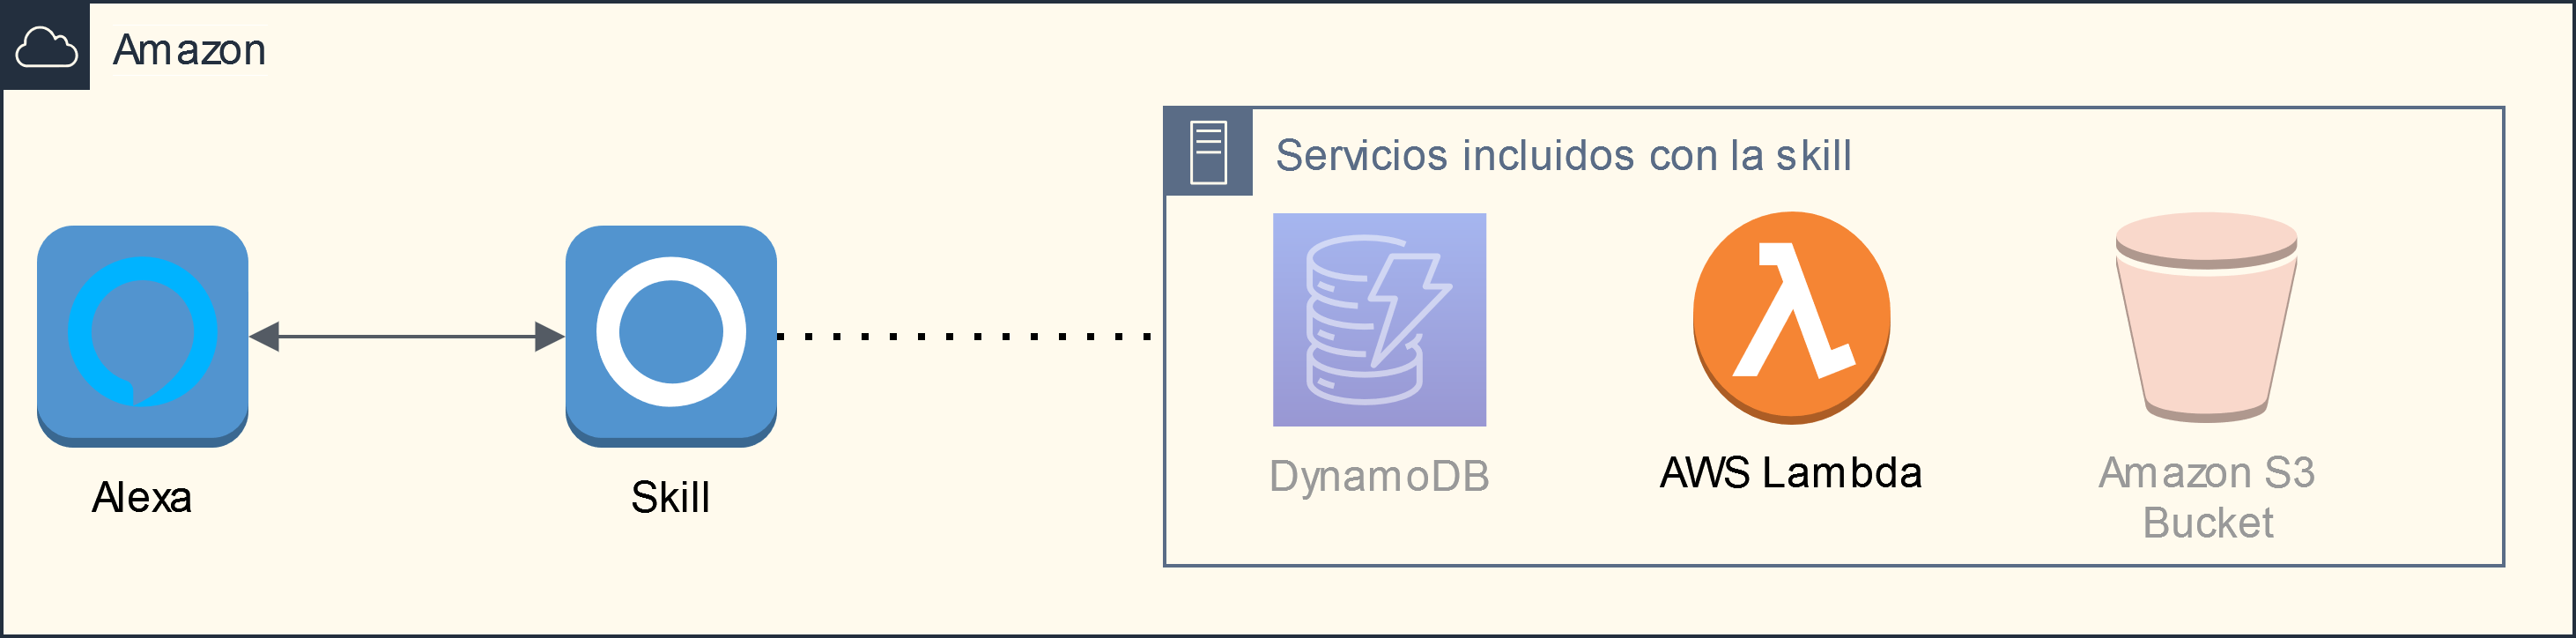
\includegraphics[width=\textwidth]{bloques-skill.png}  
  \end{frame}

  \begin{frame}{Base de datos}
    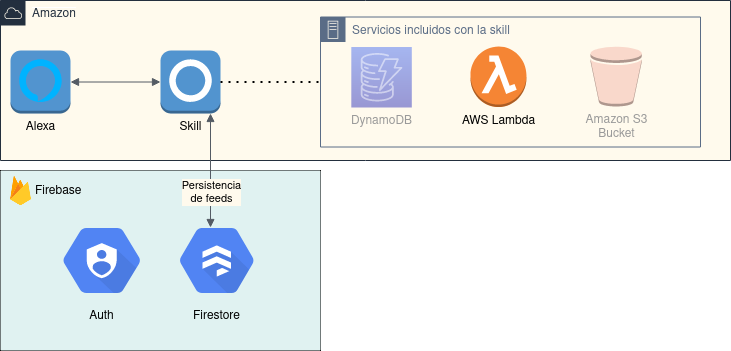
\includegraphics[width=\textwidth]{bloques-bd.png}  
  \end{frame}

  \begin{frame}{Gestión de feeds}
    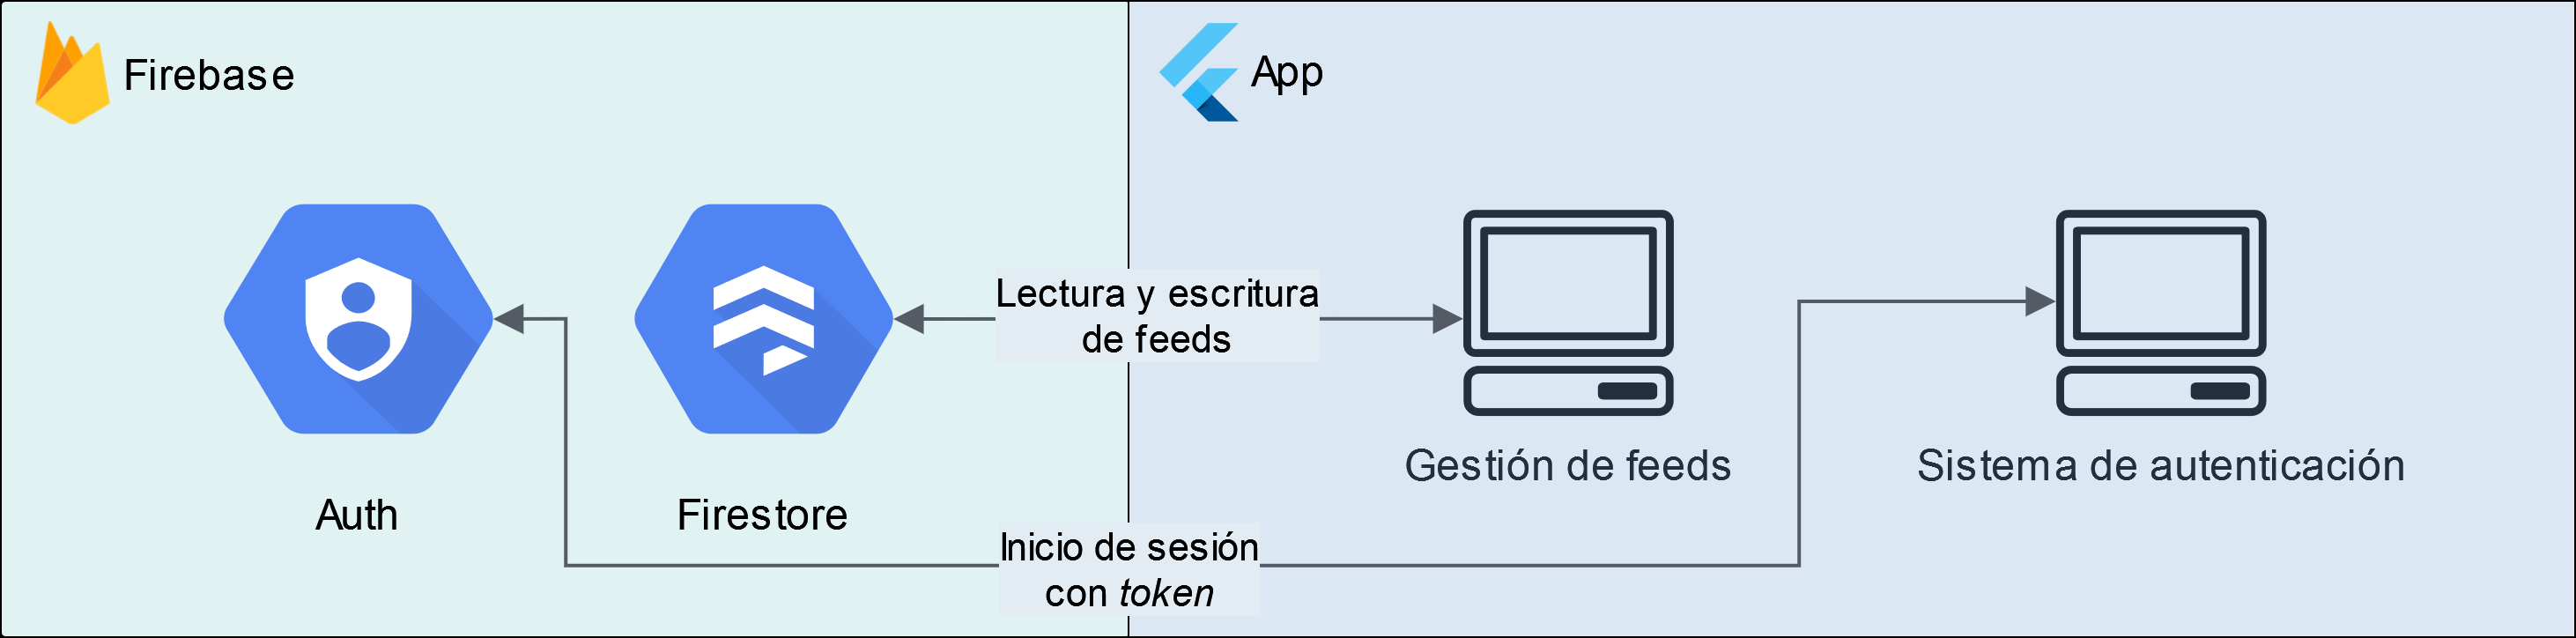
\includegraphics[width=\textwidth]{bloques-app.png}  
  \end{frame}

  \begin{frame}{Servicio de autenticación}
    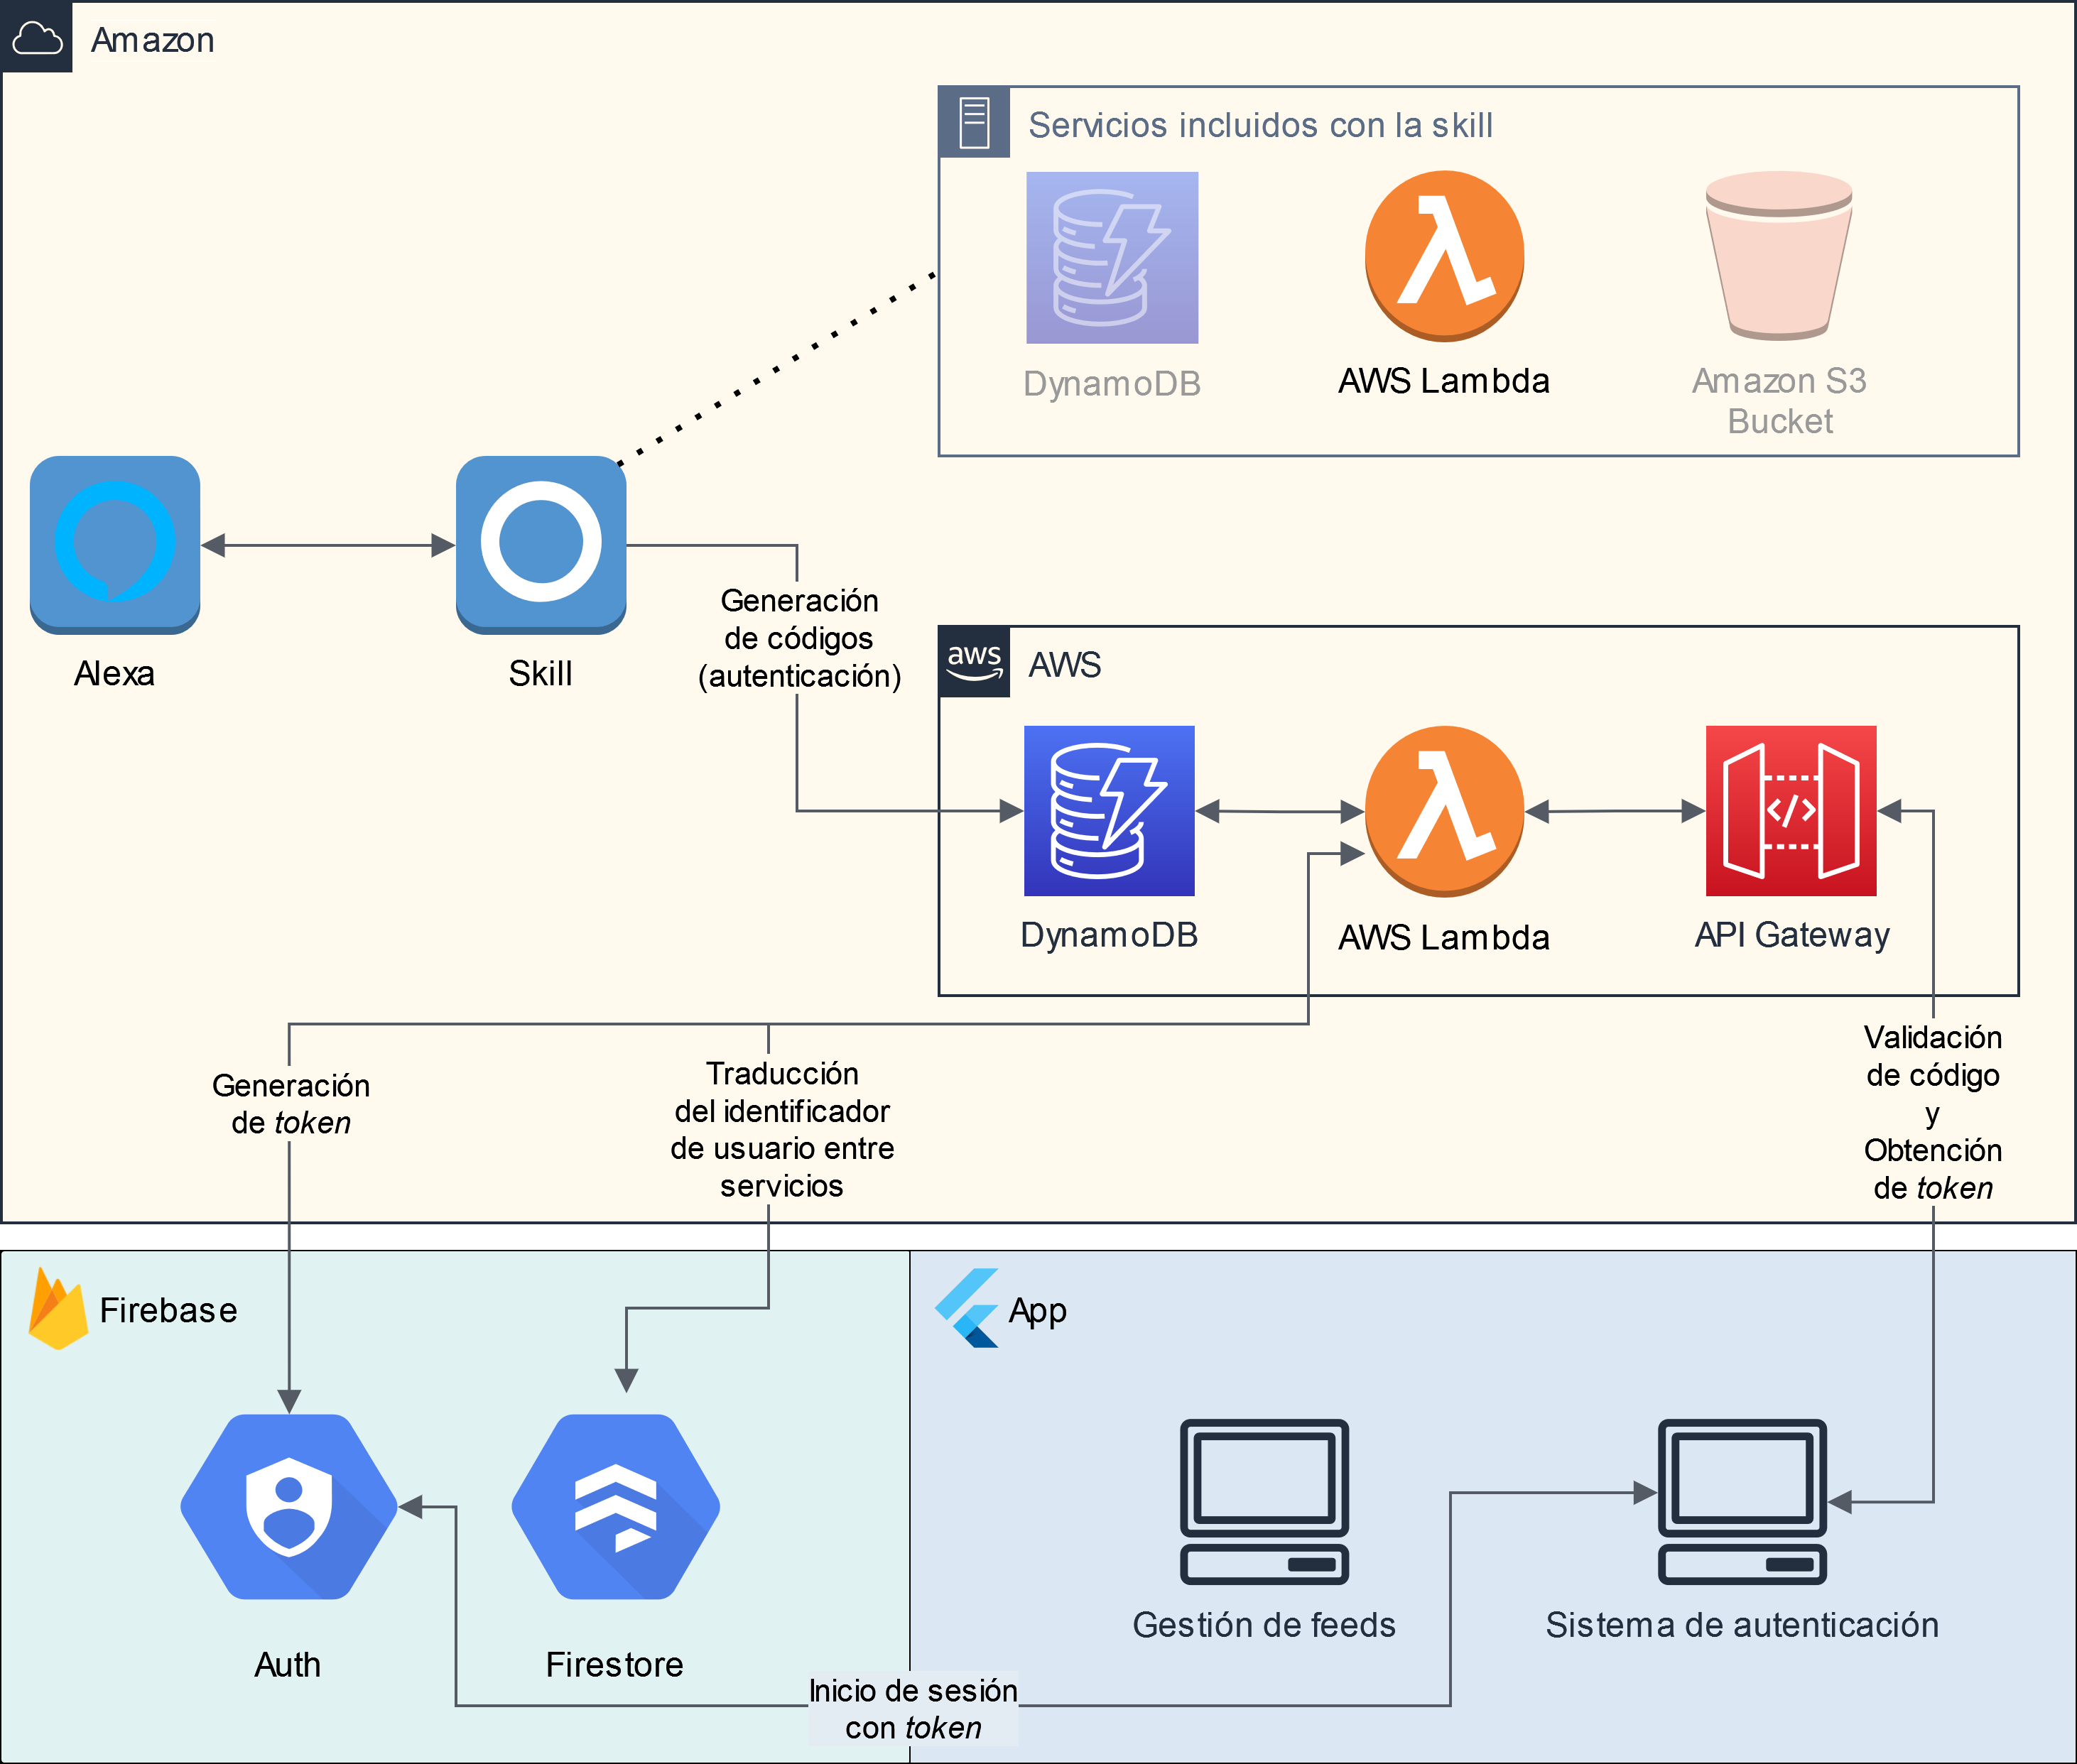
\includegraphics[width=.9\textwidth]{bloques-auth.png}  
  \end{frame}

  \begin{frame}{Resumen}
    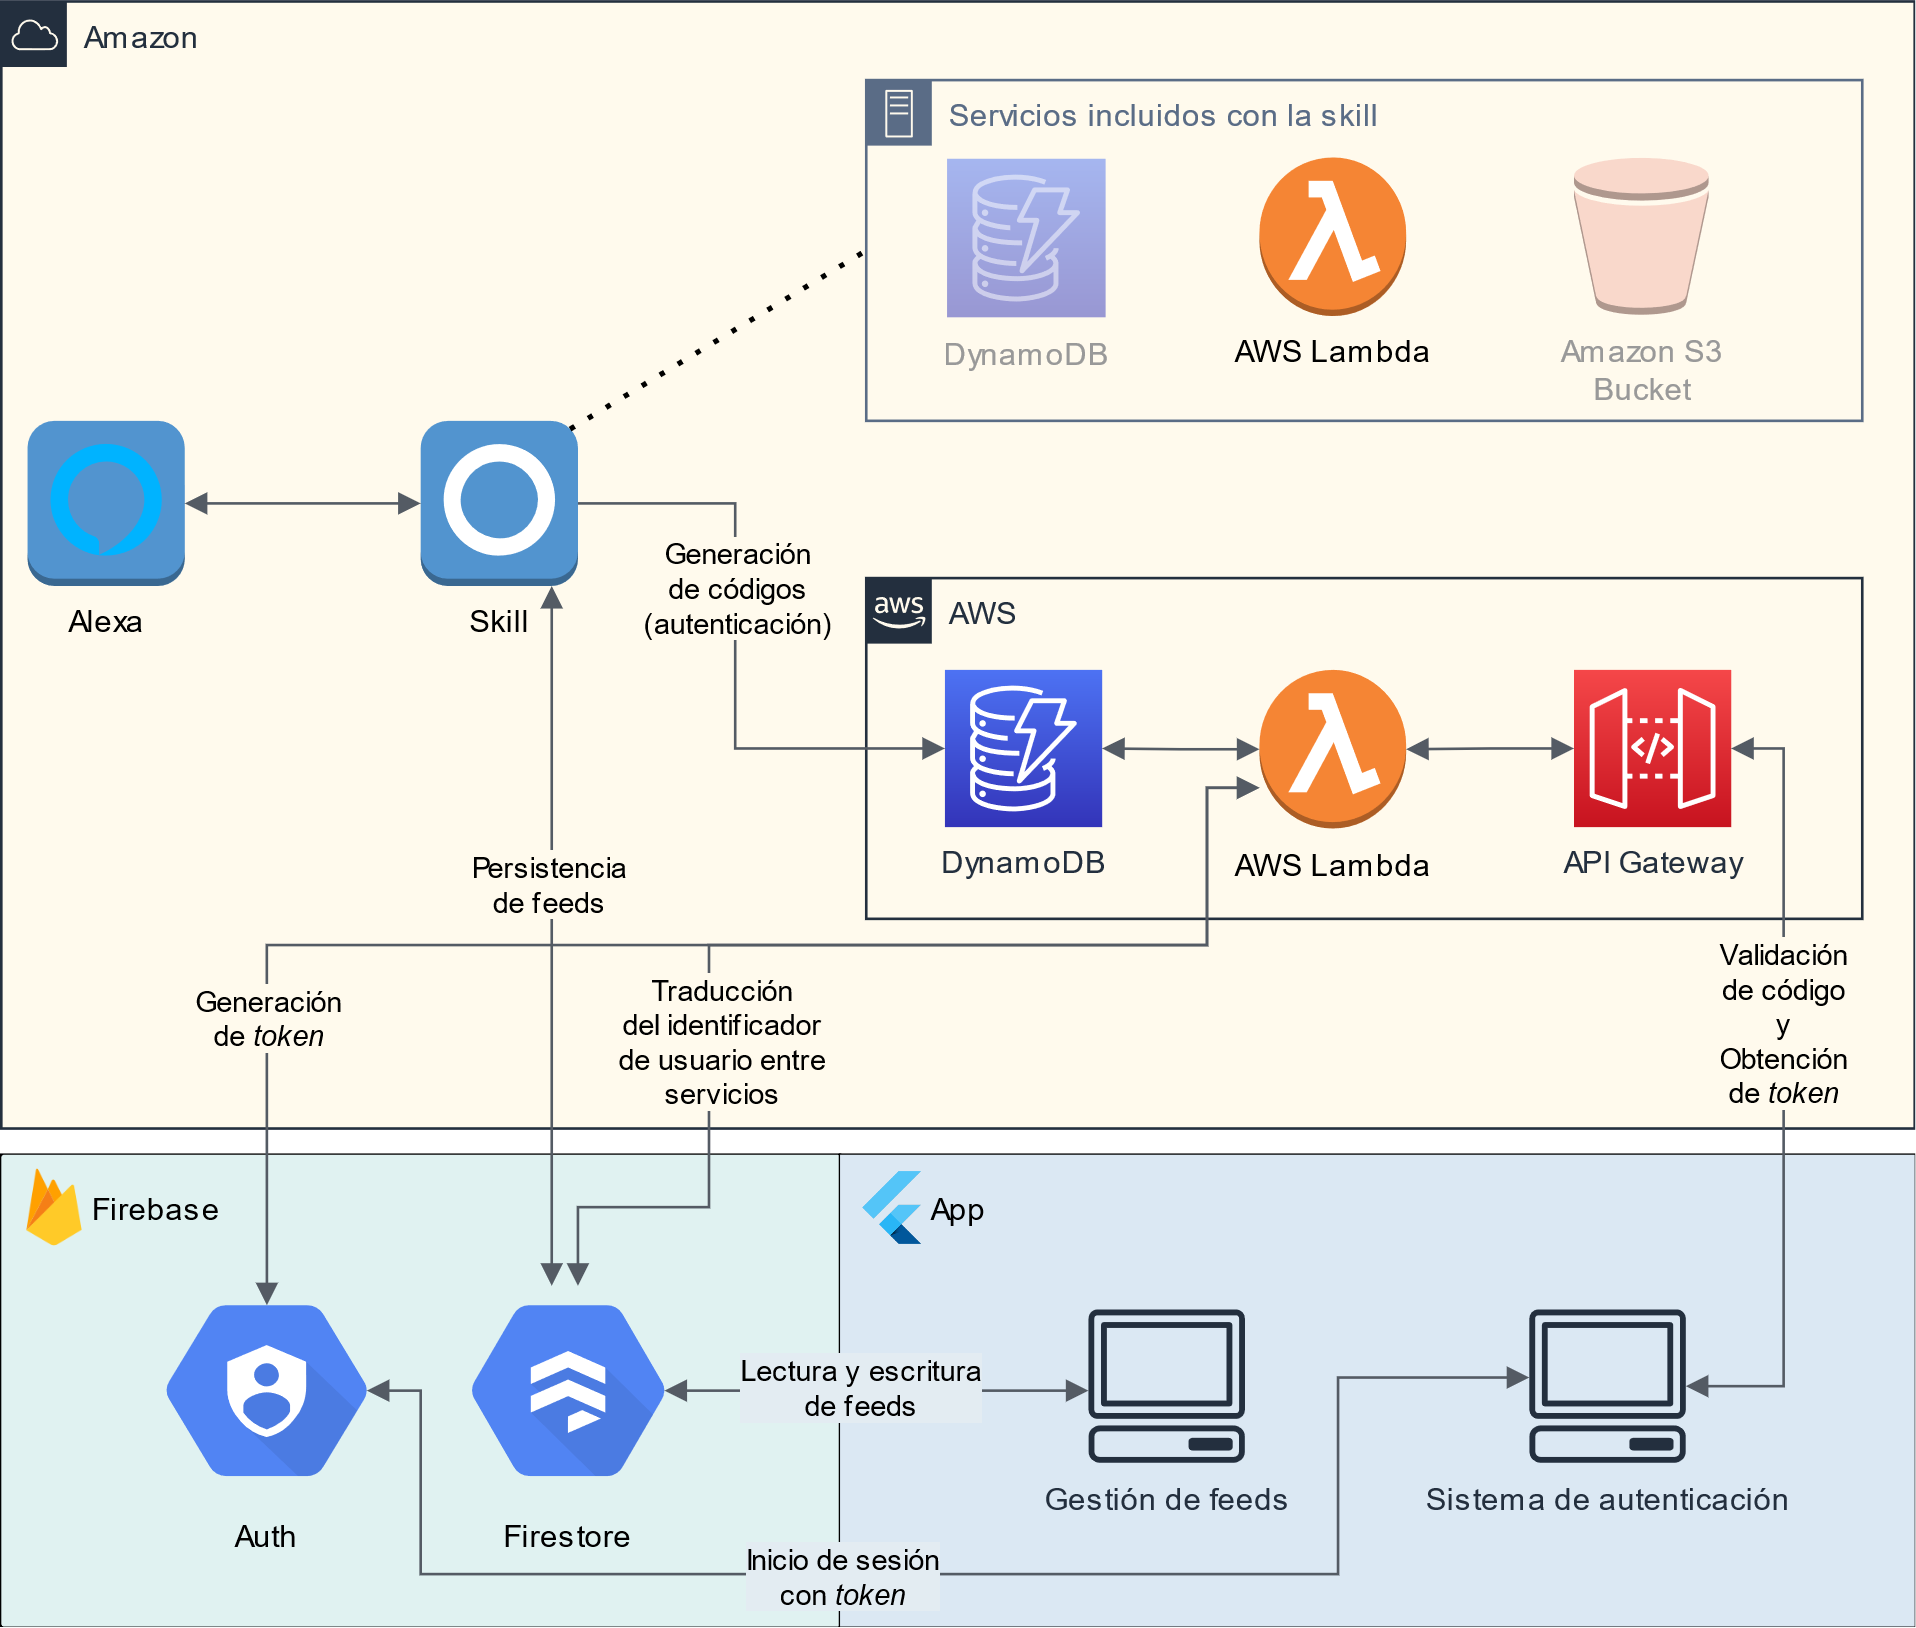
\includegraphics[width=.9\textwidth]{diagrama-bloques.png}  
  \end{frame}

  \section{Desarrollo / Implementación de la propuesta}
  
  \section{Demo}
  
  \section{Resultados obtenidos}
  
  \section{Conclusiones} % (y trabajos futuros)

\end{document}